\section{Experimental validation}

\begin{figure}[t]
    \centering
    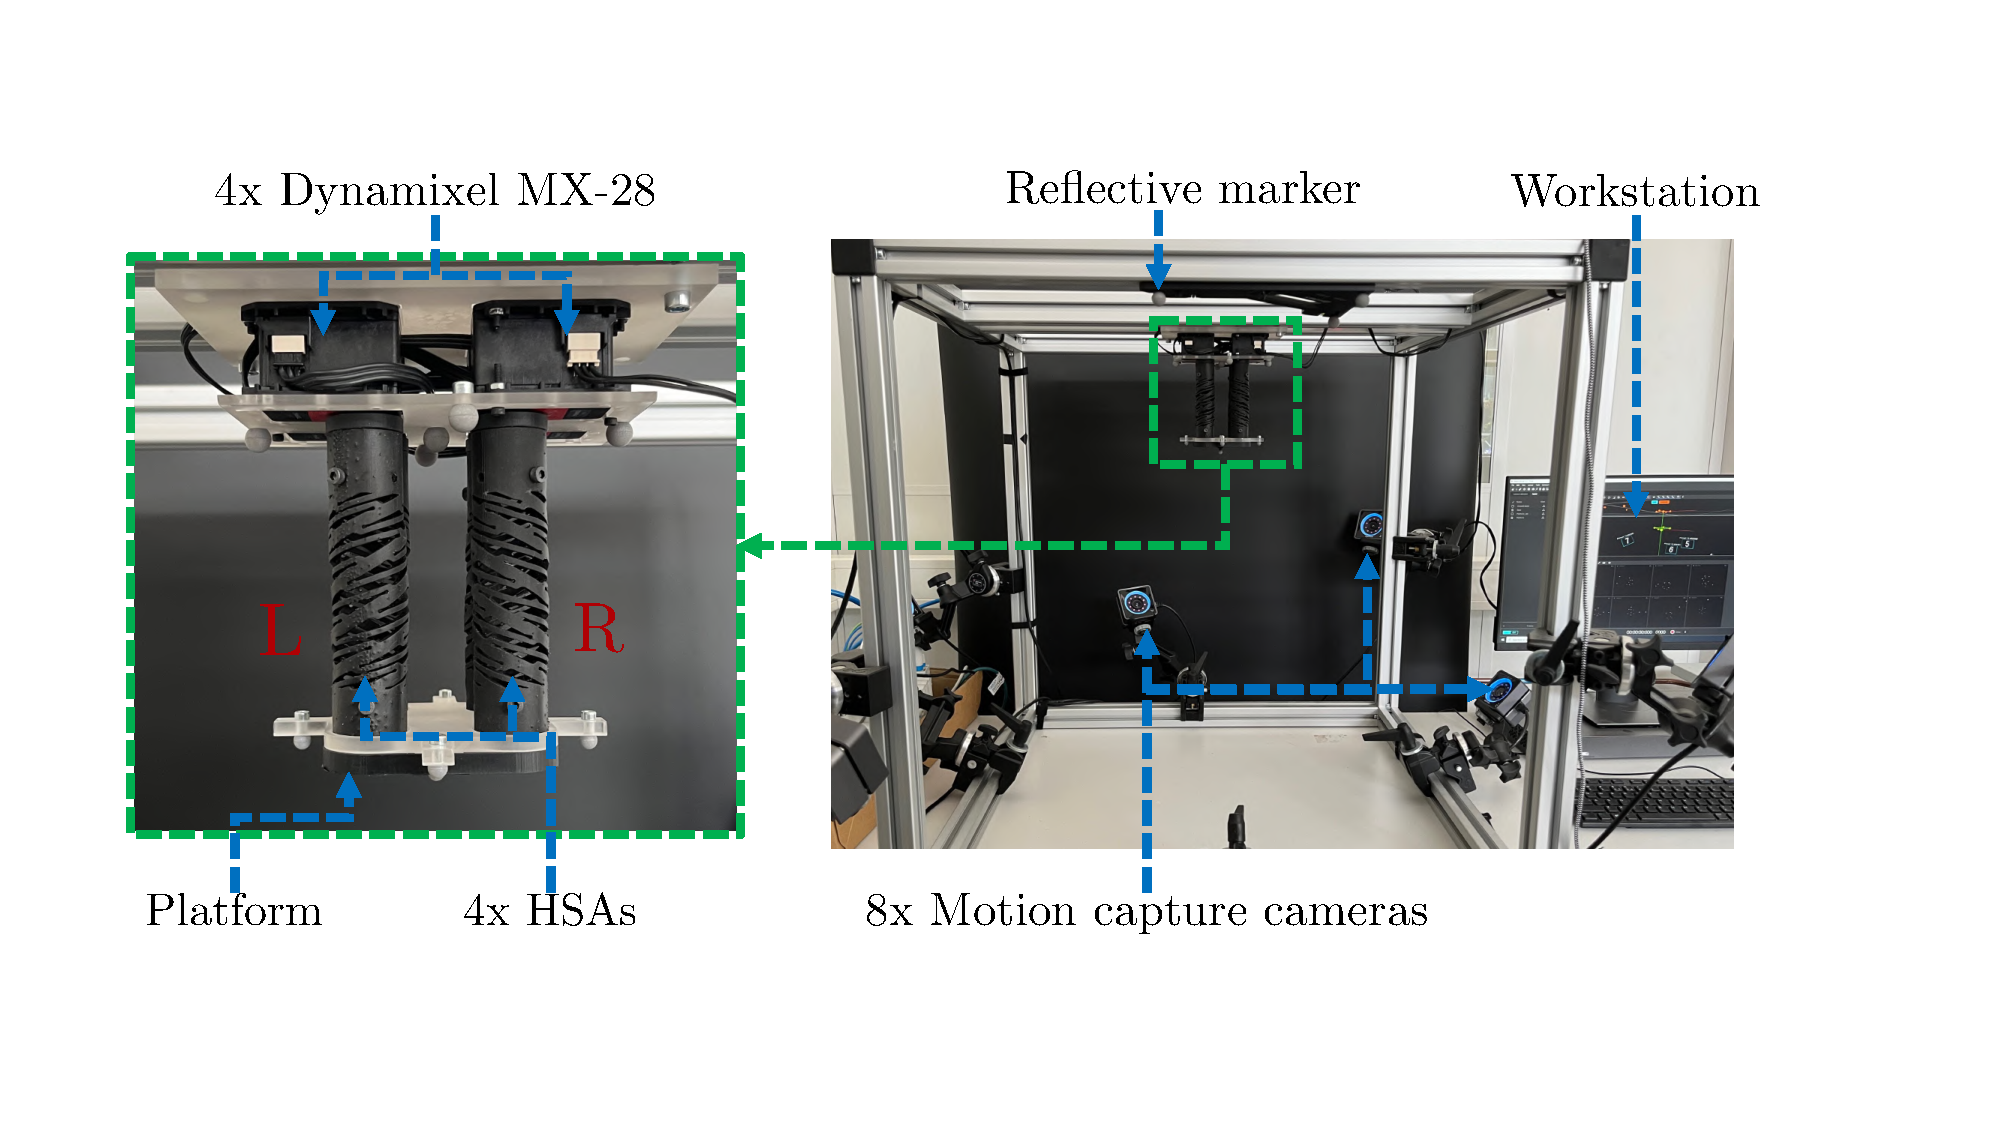
\includegraphics[width=0.85\textwidth]{hsacontrol/figures/experimental_setup_v2_cropped_compressed.pdf}
    \caption{Experimental setup: the parallel robot consists of four HSA rods connected by a platform at their distal end. Four servo motors actuate the HSAs. We track the pose of the end-effector with a motion capture system by attaching reflective markers to the platform.}
    \label{fig:hsacontrol:experimental_setup}
\end{figure}

\subsection{Experimental setup}
We evaluate the system model and our proposed control approach on a robot consisting of four HSA rods.
The material choice of the \gls{HSA} is crucial and has a significant influence on the resulting mechanical characteristics of the robot  (e.g., blocked force, holding torque, bending stiffness, etc.)~\cite{truby2021recipe}. Furthermore, specific material requirements are dictated by the nature of the design of the \gls{HSA} rod. The structure of the metamaterial is made of struts connected by living hinges. These living hinges must be thin, flexible, and accommodate high strains~\cite{truby2021recipe}.
Therefore, we decided to 3D-print the \glspl{HSA} via digital projection lithography either from the photopolymer resin Carbon FPU 50 (stiffer) or the elastomeric polyurethane EPU 40 resin (softer).
% citations for datasheets: ~\cite{carbon:fpu50} ~\cite{carbon:epu40}

Each \gls{HSA} rod is actuated by a Dynamixel MX-28 servo motor. The Dynamixel motors are set to use position control mode. % which runs a cascaded PID control loop on the motor current.
% The robot is mounted platform-down on a cage on which we have also attached eight Optitrack PrimeX 13 cameras. The motion capture system can track the SE(3) pose of both the base and the platform at a sampling rate of \SI{200}{Hz}. 
The robot is mounted platform-down on a cage with an Optitrack motion capture system, which measures the SE(3) pose of the platform at \SI{200}{Hz}.
Our algorithms run within a ROS2 framework\footnote{\url{https://github.com/tud-phi/ros2-hsa}}. % First, we project the pose measurements into the plane of actuation. Then, we evaluate the coordinate transformation between platform and base and run the closed-form inverse kinematics introduced in \eqref{eq:hsacontrol:kinematics}. We store in memory the last \textcolor{orange}{ten} configuration measurements, fit a cubic spline to each configuration variable using the \emph{Derivative} package~\cite{kaptanoglu2022pysindy}, and then differentiate the spline function to gather $\dot{q}(t)$.
% ~\footnote{\url{https://github.com/tud-phi/ros2-hsa}}
% ~\cite{kaptanoglu2022pysindy}
% Our algorithms run within a ROS2 framework. 
The pose measurements are first projected into the plane of actuation and serve as an input to the closed-form inverse kinematics introduced in \eqref{eq:hsacontrol:kinematics}. 
We use a Savitzky-Golay filter with a window duration of $\SI{0.1}{s}$ to numerically differentiate $\chi_\mathrm{ee}(t)$, $q(t)$ and gather with that $\dot{\chi}_\mathrm{ee}(t)$ and $\dot{q}(t)$.
We fit a cubic spline to the last $16$ configuration measurements and differentiate~\cite{kaptanoglu2022pysindy} to gather $\dot{q}(t)$.

\subsection{System identification}
We follow the same system identification procedure as in Sec.~\ref{sub:hsamodel:planar_hsa_robot_model:model_verification}.
For the FPU-based robot, we identify $C_\varepsilon^\mathrm{FPU}=\SI{0.0079}{m \per rad}$, $S_\mathrm{be}^\mathrm{FPU} = -2.5 \cdot 10^{-5} + 3.9 \cdot 10^{-7} \, \frac{\phi_i^+}{l^0} \si{Nm^2}$, $S_\mathrm{sh}^\mathrm{FPU} = 0.043 + 0.0029 \, \frac{\phi_i^+}{l^0} \si{N}$, $S_\mathrm{ax}^\mathrm{FPU} = 0.74 + 0.0098 \, \frac{\phi_i^+}{l^0} \si{N}$, and $S_\mathrm{b,sh}^\mathrm{FPU} = -5.0 \cdot 10^{-4} \si{Nm \per rad}$ where $l^0 = \SI{0.059}{m}$. 
Furthermore, we regress $C_\varepsilon^\mathrm{EPU}=\SI{0.0098}{m \per rad}$, $S_\mathrm{be}^\mathrm{EPU} = 5.7 \cdot 10^{-4} -9.7 \cdot 10^{-6} \, \frac{\phi_i^+}{l^0} \si{Nm^2}$, $S_\mathrm{sh}^\mathrm{EPU} = 0.59 - 0.00047 \, \frac{\phi_i^+}{l^0} \si{N}$, $S_\mathrm{ax}^\mathrm{EPU} = 5.7 + 0.015 \, \frac{\phi_i^+}{l^0} \si{N}$, and $S_\mathrm{b,sh}^\mathrm{EPU} = -\SI{0.00048}{Nm \per rad}$ for the EPU \glspl{HSA} which have the same length as the FPU \glspl{HSA}.
Finally, we identify the axial rest strain $\sigma_\mathrm{ax}^0$ before the start of each experiment.

\begin{figure}[ht]
    \centering
    \subfigure[End-effector position]{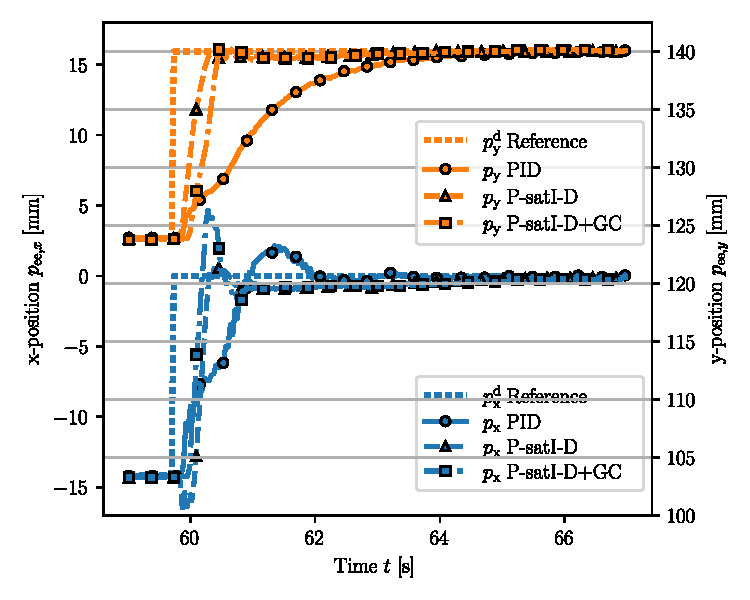
\includegraphics[width=0.49\columnwidth, trim={10, 10, 10, 10}]{hsacontrol/figures/experimental_results/fpu/fpu_step_response_chiee.pdf}\label{fig:hsacontrol:experimental_results:fpu:step_response:pee}}
    \subfigure[Configuration]{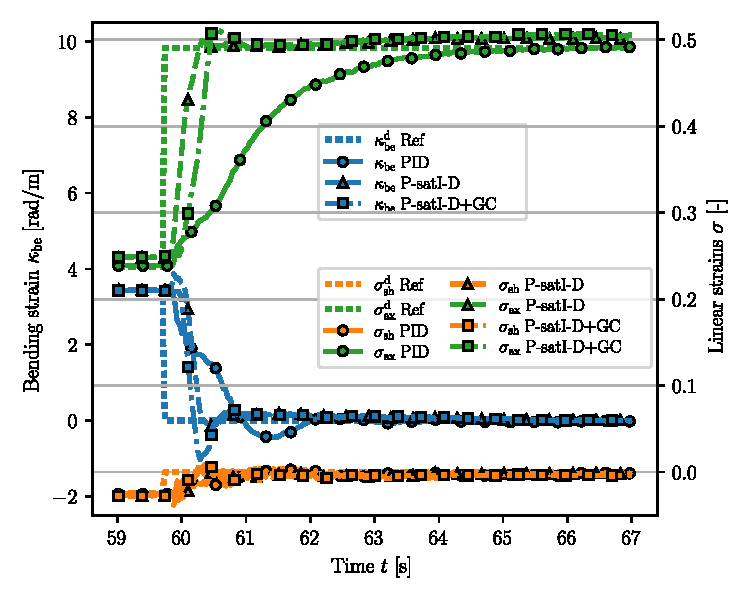
\includegraphics[width=0.49\columnwidth, trim={10, 10, 10, 10}]{hsacontrol/figures/experimental_results/fpu/fpu_step_response_q.pdf}\label{fig:hsacontrol:experimental_results:fpu:step_response:q}}
    \caption{Step response of the \emph{baseline PID}, \emph{P-satI-D} (with gravity compensation), and \emph{P-satI-D + GC} (with gravity cancellation) controllers on an FPU-based HSA robot.}\label{fig:hsacontrol:experimental_results:fpu:step_response}
\end{figure}

\begin{figure}[t]
    \centering
    \subfigure[End-effector position]{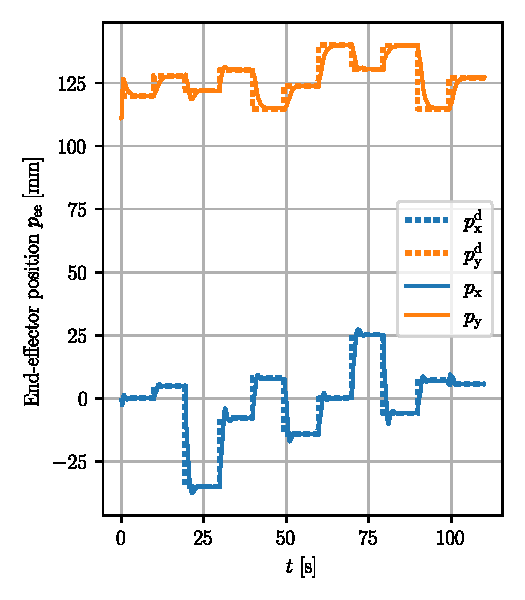
\includegraphics[width=0.32\columnwidth, trim={10, 10, 5, 10}]{hsacontrol/figures/experimental_results/fpu/20230925_092200_pee_three_panel_layout.pdf}\label{fig:hsacontrol:experimental_results:fpu:baseline_pid:pee}}
    \subfigure[Configuration]{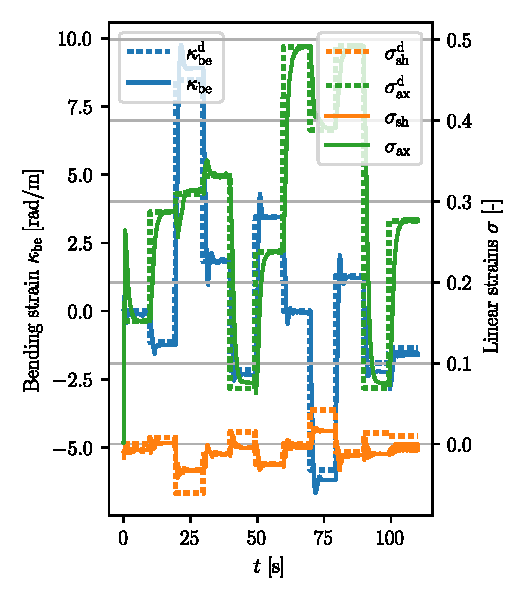
\includegraphics[width=0.32\columnwidth, trim={10, 10, 10, 10}]{hsacontrol/figures/experimental_results/fpu/20230925_092200_q_three_panel_layout.pdf}\label{fig:hsacontrol:experimental_results:fpu:baseline_pid:q}}
    \subfigure[Control input]{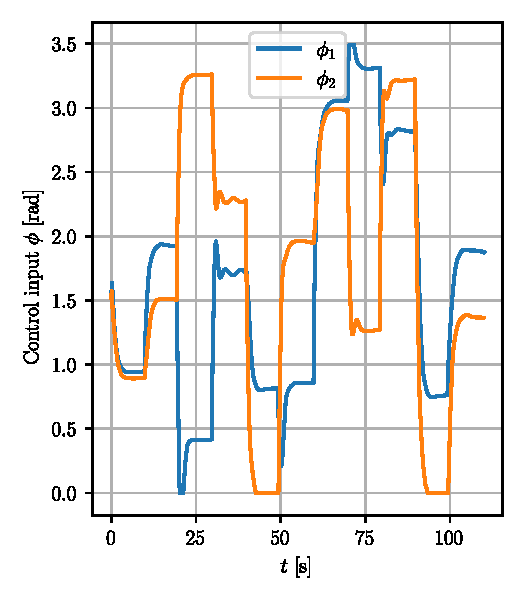
\includegraphics[width=0.32\columnwidth, trim={10, 10, 10, 10}]{hsacontrol/figures/experimental_results/fpu/20230925_092200_phi_three_panel_layout.pdf}\label{fig:hsacontrol:experimental_results:fpu:baseline_pid:phi}}
    \caption{Experimental results for tracking a reference trajectory of eleven step functions with the baseline PID controller on an FPU-based HSA robot. \textbf{Panel (a):} End-effector position with the dotted and solid lines denoting the task-space reference and actual position, respectively.
    \textbf{Panel (b):} The planned (dotted) and the actual (solid) configuration. 
    \textbf{Panel (c):} The planned (dotted) and the actual (solid) actuation coordinates of the collocated system. 
    \textbf{Panel(d):} The saturated planar control inputs are visualized with solid lines, and the computed steady-state actuation with dotted lines.}\label{fig:hsacontrol:experimental_results:fpu:baseline_pid}
\end{figure}

\subsection{Steady-state planning}\label{sub:hsacontrol:experiments:steady_state_planning}
Our approach, as detailed in Section~\ref{sub:hsacontrol:methodology:control}, requires us for a given desired end-effector position $p_\mathrm{ee}^\mathrm{d}$ to identify a statically-feasible configuration $q^\mathrm{d}$ with the matching steady-state actuation $\phi^\mathrm{ss}$.

We perform online static inversion to identify admittable desired configurations $q^\mathrm{d}$ and matching steady-state control inputs $\phi^\mathrm{ss}$ during our experiments involving the FPU \gls{HSA} robots. First, we substitute the inverse kinematics $\varrho_\mathrm{ee}(\chi_\mathrm{ee})$ into the static \gls{EOM}. Then, we find the roots of the equation $G\circ\varrho_\mathrm{ee}(\chi_\mathrm{ee}^\mathrm{d}) + K\circ\varrho_\mathrm{ee}(\chi_\mathrm{ee}^\mathrm{d})-\alpha(\varrho_\mathrm{ee}(\chi_\mathrm{ee}^\mathrm{d}), \phi_\mathrm{ss})$ with respect to $(\theta_\mathrm{ee},\phi_1, \phi_2)$ using nonlinear least-squares while enforcing constraints on the sign of $\phi$. We solve this optimization problem with projected gradient descent.

In contrast, the static inversion optimization problem is not well-behaved for the identified EPU system parameters. Instead, we rely on rolling out the dynamics over a duration $t_\mathrm{ss}$ to steady-state and then optimize the steady-state input $\phi^\mathrm{ss}$ such that the final end-effector error $\lVert p_\mathrm{ee}^\mathrm{d} - p_\mathrm{ee}^\mathrm{ss} \rVert$ is as small as possible. We formalize this optimization problem in a least-squares fashion
\begin{equation}\label{eq:hsacontrol:steady_state_rollout_optim_problem}
\begin{aligned}
    \phi^\mathrm{ss} = \argmin_\mathrm{\phi} \quad & \frac{1}{2} \, \lVert p_\mathrm{ee}^\mathrm{d} - p_\mathrm{ee}^\mathrm{ss}(\phi) \rVert_2^2,\\
    \textrm{s.t.} \quad & x^\mathrm{ss} = x(t_0) + \int_{t_0}^{t_\mathrm{ss}} f(x(t), \phi) \, \mathrm{d}t, \quad \chi_\mathrm{ee}^\mathrm{ss} = \begin{bmatrix}
        p_\mathrm{ee}^\mathrm{ss}\\
        \theta_\mathrm{ee}^\mathrm{ss}
    \end{bmatrix} = \pi_\mathrm{ee}(q^\mathrm{ss}),\\
\end{aligned}
\end{equation}
where $\dot{x}(t) = f(x(t), \phi)$ are the nonlinear state-space dynamics based on the \gls{EOM} derived in Section~\ref{sub:hsacontrol:methodology:dynamics} and $\phi \in \mathbb{R}^2$ is constant in time. We solve \eqref{eq:hsacontrol:steady_state_rollout_optim_problem} online using the Levenberg-Marquardt algorithm. Finally, we choose $q^d = q^\mathrm{ss}$ and $\chi_\mathrm{ee}^\mathrm{d} = \pi_\mathrm{ee}(q^d)$.

\subsection{Closed-loop control}
Next, we implement the closed-loop control strategy laid out in Section~\ref{sub:hsacontrol:methodology:control}.
After evaluating the control law at a rate of \SI{40}{Hz} and saturating the control inputs to the ranges $[0, 3.40] \, \si{rad}$ for FPU and $[0, 4.71] \, \si{rad}$ for EPU, respectively, we map $\phi \in \mathbb{R}^2$ to desired positions of the four motors. For this, we consider the handedness of the \glspl{HSA} and apply the same actuation magnitude to both rods on the same side of the virtual backbone.
After tuning the gains for the feedback part of the model-based control laws in \eqref{eq:hsacontrol:gravity_compensation_controller} and \eqref{eq:hsacontrol:gravity_cancellation_controller}, we select $K_\mathrm{p} = \mathrm{diag}(0.3, 0.3)$, $K_\mathrm{i} = \mathrm{diag}(0.05, 0.05) \, \si{1 \per s}$, $K_\mathrm{d} = \mathrm{diag}(0.01, 0.01) \, \si{s}$, and $\gamma = \mathrm{diag}(100, 100)$. 
Furthermore, we report the performance of a model-free PID controller as a baseline. Here, the control input in task-space is given by $u_\mathrm{ts} = \begin{bmatrix}u_\mathrm{ts,x} & u_\mathrm{ts,y}\end{bmatrix}^\mathrm{T} = K_\mathrm{p}^\mathrm{PID} \, (p_\mathrm{ee}^\mathrm{d}-p_\mathrm{ee}) - K_\mathrm{d}^\mathrm{PID} \, \dot{p}_\mathrm{ee} + K_\mathrm{i}^\mathrm{PID} \int_0^t p_{\mathrm{ee},t'}^\mathrm{d} - p_{\mathrm{ee},t'} \: \mathrm{d}t'$, which is then mapped to the actuation via $\phi = \begin{bmatrix}
    u_\mathrm{ts,x}+u_\mathrm{ts,y}, & -u_\mathrm{ts,x}+u_\mathrm{ts,y}
\end{bmatrix}^\mathrm{T}$.
Here, we select $K_\mathrm{p}^\mathrm{PID} = \mathrm{diag}(10, 10) \, \si{rad \per m}$, $ K_\mathrm{i}^\mathrm{PID} = \mathrm{diag}(110, 110) \, \si{rad \per \meter \per \second}$, and $ K_\mathrm{d}^\mathrm{PID} = \mathrm{diag}(0.25, 0.25) \, \si{rad \, \second \per \meter}$.
\\

\begin{figure}[ht]
    \centering
    \subfigure[End-effector position]{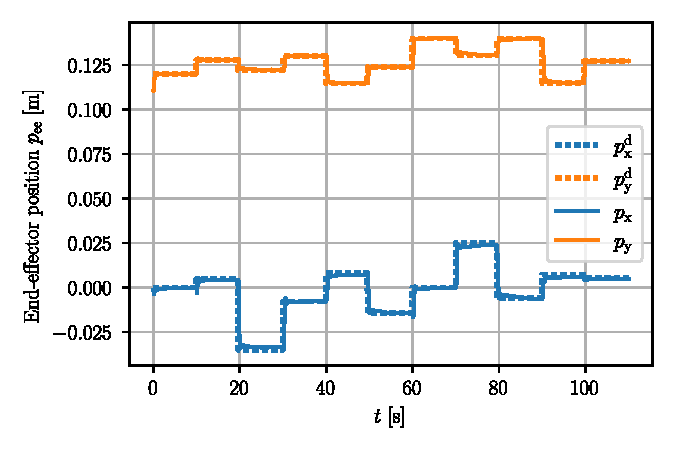
\includegraphics[width=0.49\columnwidth, trim={5, 10, 5, 5}]{hsacontrol/figures/experimental_results/fpu/20230925_093236_pee.pdf}\label{fig:hsacontrol:experimental_results:fpu:p_sati_d:pee}}
    \subfigure[Configuration]{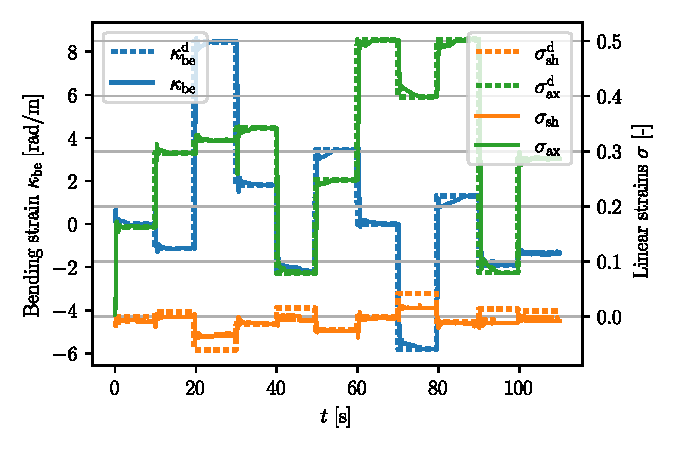
\includegraphics[width=0.49\columnwidth, trim={5, 10, 5, 5}]{hsacontrol/figures/experimental_results/fpu/20230925_093236_q.pdf}\label{fig:hsacontrol:experimental_results:fpu:p_sati_d:q}}\\
    \subfigure[Actuation coordinates]{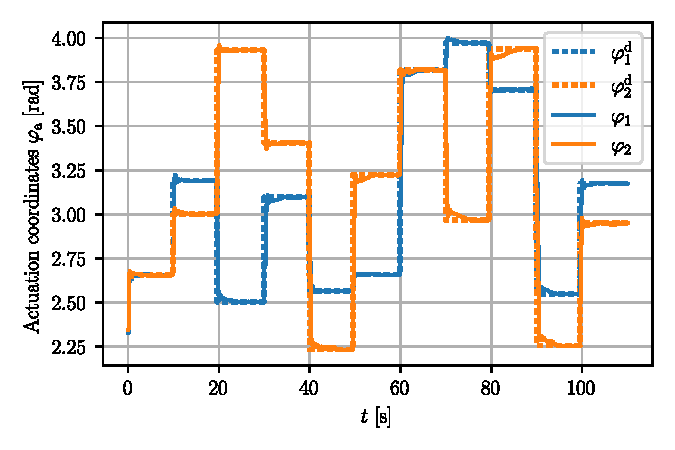
\includegraphics[width=0.49\columnwidth, trim={5, 10, 5, 5}]{hsacontrol/figures/experimental_results/fpu/20230925_093236_varphi.pdf}\label{fig:hsacontrol:experimental_results:fpu:p_sati_d:varphi}}
    \subfigure[Control input]{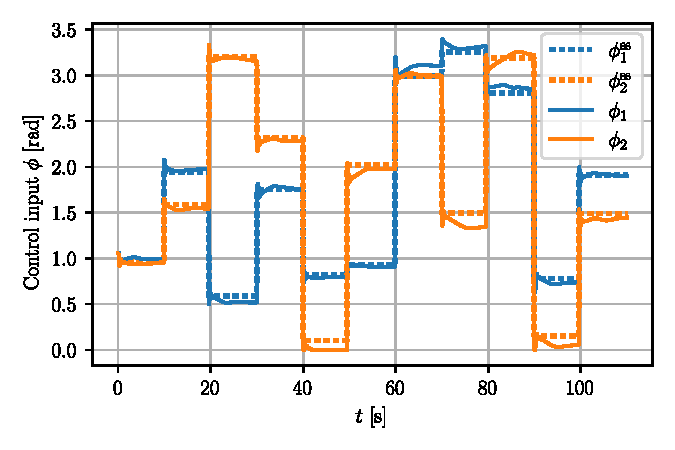
\includegraphics[width=0.49\columnwidth, trim={5, 10, 5, 5}]{hsacontrol/figures/experimental_results/fpu/20230925_093236_phi.pdf}\label{fig:hsacontrol:experimental_results:fpu:p_sati_d:phi}}\\
    \caption{Experimental results for tracking a reference trajectory of eleven step functions with the P-satI-D controller on an FPU-based HSA robot. \textbf{Panel (a):} End-effector position with the dotted and solid lines denoting the task-space reference and actual position, respectively.
    \textbf{Panel (b):} The planned (dotted) and the actual (solid) configuration. 
    \textbf{Panel (c):} The planned (dotted) and the actual (solid) actuation coordinates of the collocated system. 
    \textbf{Panel(d):} The saturated planar control inputs are visualized with solid lines, and the computed steady-state actuation with dotted lines.}\label{fig:hsacontrol:experimental_results:fpu:p_sati_d}
\end{figure}

\begin{figure}[ht]
    \centering
    \subfigure[End-effector position]{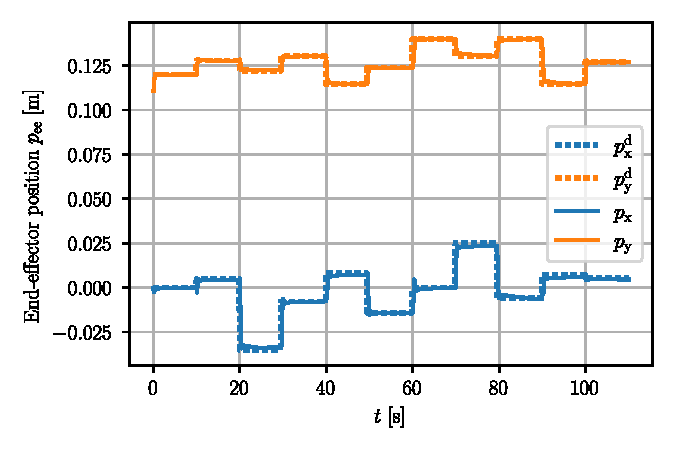
\includegraphics[width=0.49\columnwidth, trim={5, 5, 5, 5}]{hsacontrol/figures/experimental_results/fpu/20230925_094023_pee.pdf}\label{fig:hsacontrol:experimental_results:fpu:p_sati_d_plus_gc:pee}}
    \subfigure[Configuration]{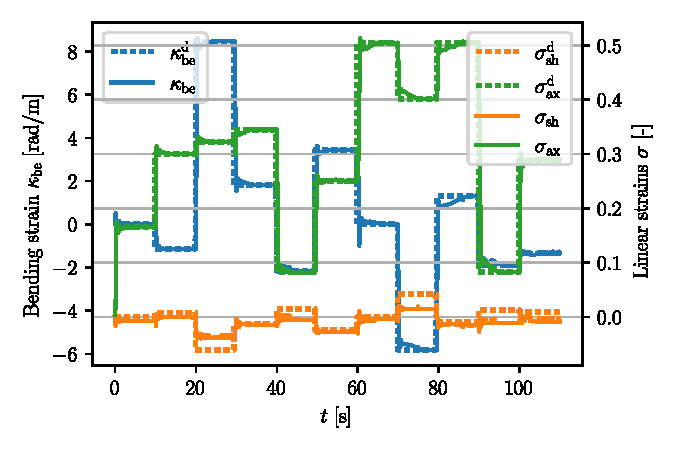
\includegraphics[width=0.49\columnwidth, trim={5, 5, 5, 5}]{hsacontrol/figures/experimental_results/fpu/20230925_094023_q.pdf}\label{fig:hsacontrol:experimental_results:fpu:p_sati_d_plus_gc:q}}\\
    \subfigure[Actuation coordinates]{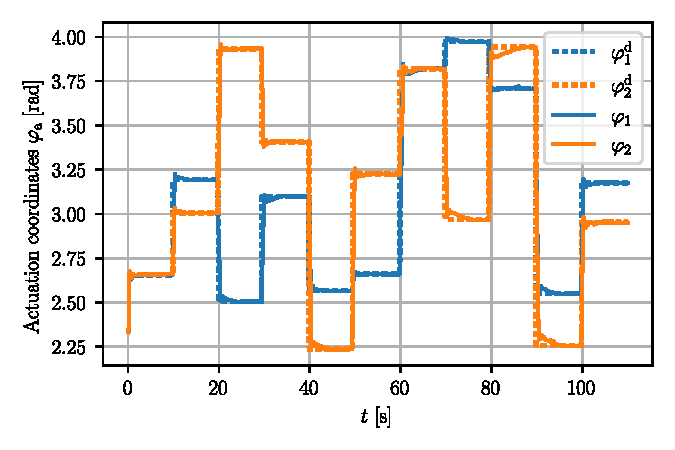
\includegraphics[width=0.49\columnwidth, trim={5, 5, 5, 5}]{hsacontrol/figures/experimental_results/fpu/20230925_094023_varphi.pdf}\label{fig:hsacontrol:experimental_results:fpu:p_sati_d_plus_gc:varphi}}
    \subfigure[Control input]{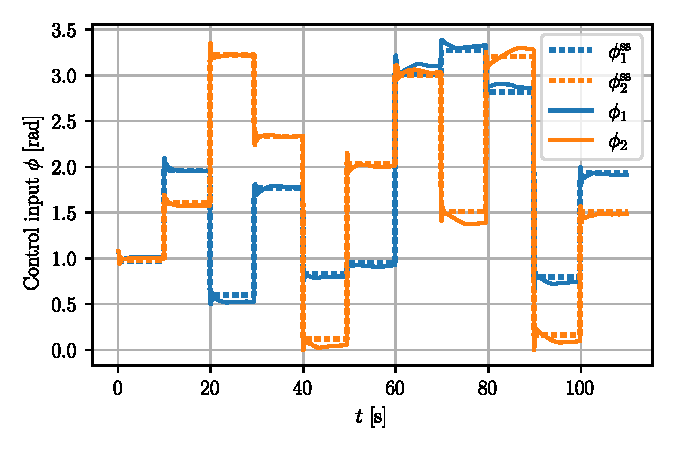
\includegraphics[width=0.49\columnwidth, trim={5, 5, 5, 5}]{hsacontrol/figures/experimental_results/fpu/20230925_094023_phi.pdf}\label{fig:hsacontrol:experimental_results:fpu:p_sati_d_plus_gc:phi}}\\
    \caption{Experimental results for tracking a reference trajectory of eleven step functions with the P-satI-D + gravity cancellation controller on an FPU-based HSA robot. \textbf{Panel (a):} End-effector position with the dotted and solid lines denoting the task-space reference and actual position, respectively.
    \textbf{Panel (b):} The planned (dotted) and the actual (solid) configuration. 
    \textbf{Panel (c):} The planned (dotted) and the actual (solid) actuation coordinates of the collocated system. 
    \textbf{Panel(d):} The saturated planar control inputs are visualized with solid lines and the computed steady-state actuation with dotted lines.}\label{fig:hsacontrol:experimental_results:fpu:p_sati_d_plus_gc}
\end{figure}

\subsubsection{Evaluation}
We define a reference trajectory $p_\mathrm{ee}^\mathrm{d}(k), k \in \{ 1, \dots, n_k \}$ with a duration of \SI{110}{s} and consisting of eleven step functions as the reference trajectory.
We report the \gls{RMSE} metric $\sqrt{\sum_{k=1}^{n_k} \frac{\lVert p_\mathrm{ee}^\mathrm{d}(k) - p_\mathrm{ee}(k) \rVert_2^2}{n_k}}$ for assessing the control performance, where $p_\mathrm{ee}(k)$ is the actual trajectory of the end-effector.\\

\subsubsection{Control of an FPU-based HSA robot}
The \emph{baseline PID} achieves an \gls{RMSE} of \SI{5.86}{mm} with respect to the reference trajectory. The \emph{P-satI-D} based on \eqref{eq:hsacontrol:gravity_compensation_controller} (with gravity compensation) exhibits an RMSE of \SI{4.17}{mm}. Similarly, the \emph{P-satI-D + GC} based on \eqref{eq:hsacontrol:gravity_cancellation_controller} (with gravity cancellation) displays an RMSE of \SI{4.13}{mm}.
We present a comparison of the three different controllers for a step response in Fig.~\ref{fig:hsacontrol:experimental_results:fpu:step_response} and plot the entire trajectories of the \emph{baseline PID} and the \emph{P-satI-D} in Figures~\ref{fig:hsacontrol:experimental_results:fpu:baseline_pid} and \ref{fig:hsacontrol:experimental_results:fpu:p_sati_d}, respectively.
Additionally, we discretize various continuous reference trajectories into setpoints: 
star trajectory ($873$ setpoints and duration of \SI{109}{s}), the flame of the TU Delft logo ($680$ setpoints and duration of \SI{85}{s}), the contour of the MIT-CSAIL logo ($1046$ setpoints and duration of \SI{131}{s}), and the outline of a bat at three different sizes ($1510$ setpoints and \SI{189}{s} duration).
The resulting Cartesian evolutions of the \emph{P-satI-D} controller tracking these continuous references are displayed in Fig.~\ref{fig:hsacontrol:experimental_results:fpu:task_space_trajectories}.

\begin{figure}[ht]
    \centering
    \subfigure[Star]{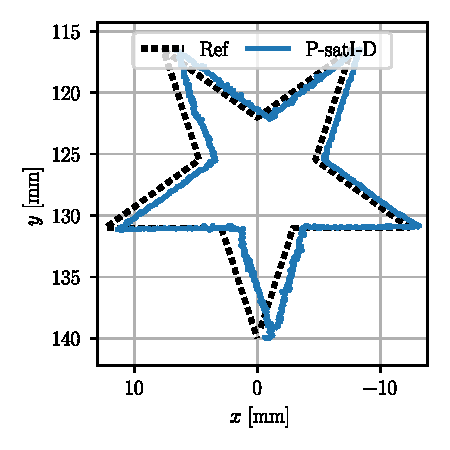
\includegraphics[width=0.32\columnwidth, trim={5, 5, 5, 5}]{hsacontrol/figures/experimental_results/fpu/20231019_072747_cartesian_evolution.pdf}\label{fig:hsacontrol:experimental_results:fpu:star}}
    \subfigure[TUD flame]{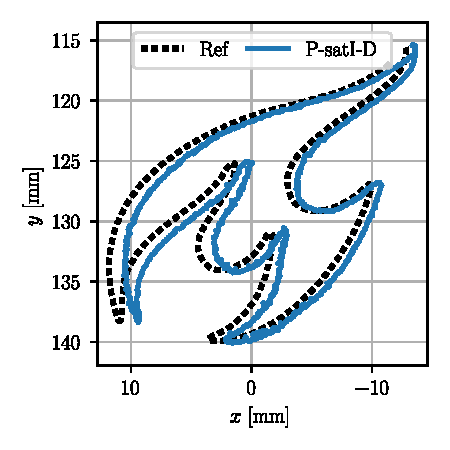
\includegraphics[width=0.32\columnwidth, trim={5, 5, 5, 5}]{hsacontrol/figures/experimental_results/fpu/20231019_081703_cartesian_evolution.pdf}\label{fig:hsacontrol:experimental_results:fpu:tud_flame}}
    \subfigure[MIT-CSAIL]{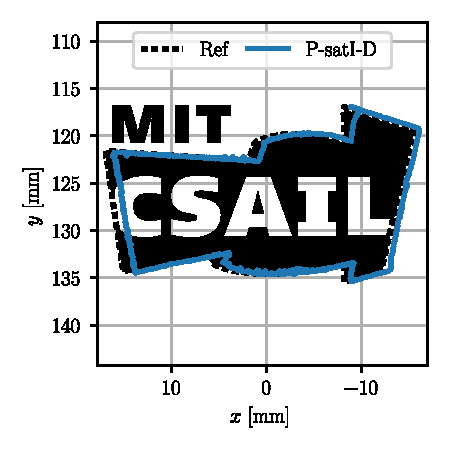
\includegraphics[width=0.32\columnwidth, trim={5, 5, 5, 5}]{hsacontrol/figures/experimental_results/fpu/20231019_082343_cartesian_evolution_with_logo.pdf}\label{fig:hsacontrol:experimental_results:fpu:mit_csail}}\\
    \subfigure[Bat trajectories]{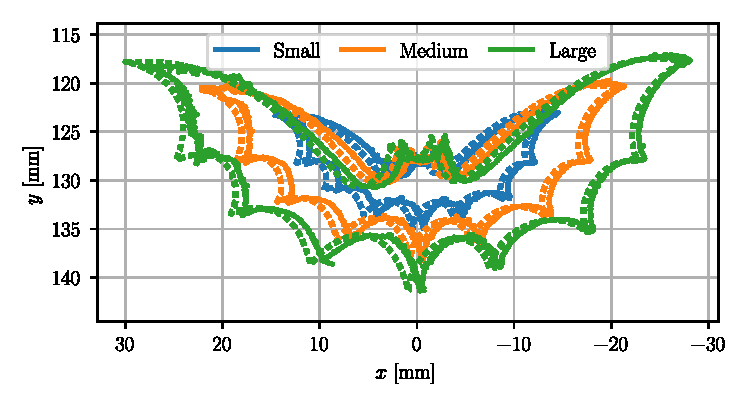
\includegraphics[width=0.7\columnwidth, trim={5, 5, 5, 5}]{hsacontrol/figures/experimental_results/fpu/fpu_bats.pdf}\label{fig:hsacontrol:experimental_results:fpu:bats}}
    \caption{Cartesian evolution of the proposed P-sat-D controller (solid lines) tracking various continuous reference trajectories (dotted lines) on the FPU robot.
    % we compare the performance of the baseline PID, the model-based P-satI-D controller (with gravity compensation), P-satI-D + GC which also includes terms to cancel the gravitational effects.
    }\label{fig:hsacontrol:experimental_results:fpu:task_space_trajectories}
\end{figure}

\begin{figure}[hb]
    \centering
    % each picture has a size 575x575px
    \subfigure[t=\SI{0}{s}]{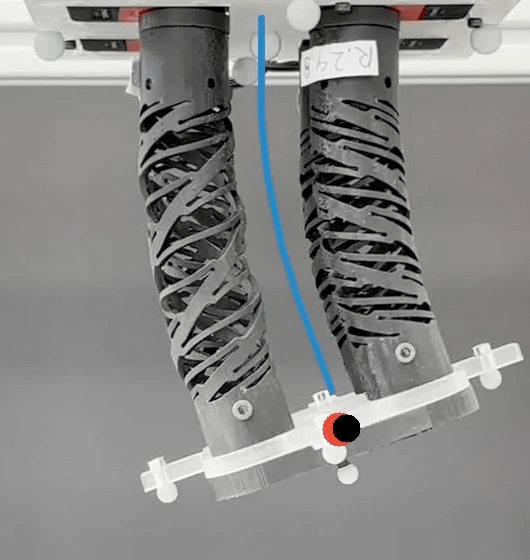
\includegraphics[width=0.192\columnwidth]{hsacontrol/figures/sequence_of_stills/bat_large/20231019_083240_overlayed_600x_cropped-0001-min.png}}
    \subfigure[t=\SI{47}{s}]{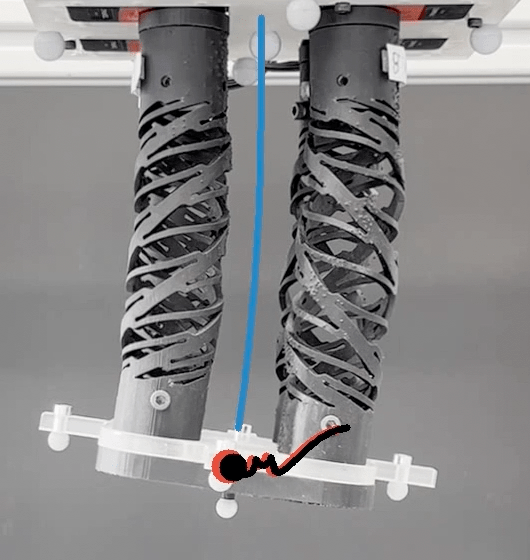
\includegraphics[width=0.192\columnwidth]{hsacontrol/figures/sequence_of_stills/bat_large/20231019_083240_overlayed_600x_cropped-0002-min.png}}
    \subfigure[t=\SI{94}{s}]{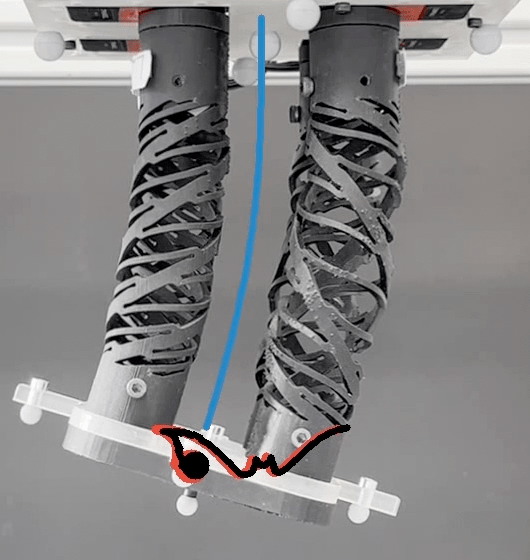
\includegraphics[width=0.192\columnwidth]{hsacontrol/figures/sequence_of_stills/bat_large/20231019_083240_overlayed_600x_cropped-0003-min.png}}
    \subfigure[t=\SI{141}{s}]{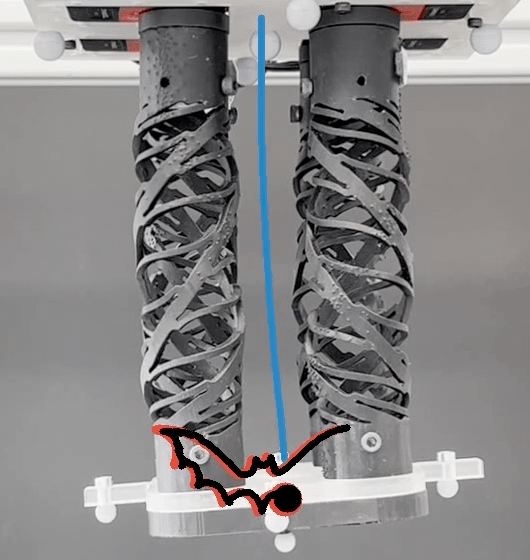
\includegraphics[width=0.192\columnwidth]{hsacontrol/figures/sequence_of_stills/bat_large/20231019_083240_overlayed_600x_cropped-0004-min.png}}
    \subfigure[t=\SI{188}{s}]{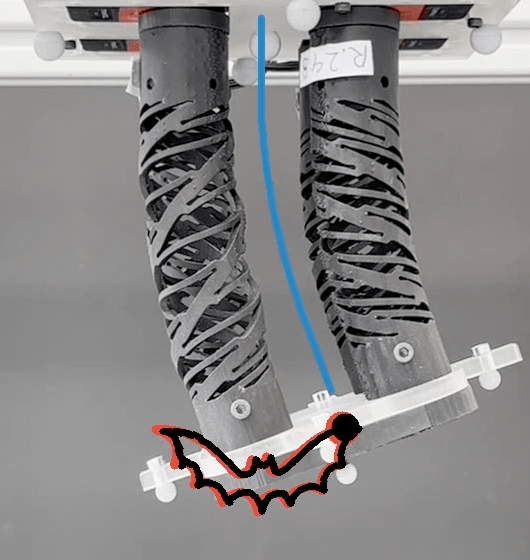
\includegraphics[width=0.192\columnwidth]{hsacontrol/figures/sequence_of_stills/bat_large/20231019_083240_overlayed_600x_cropped-0005-min.png}}
    \caption{Sequence of stills for the large bat trajectory performed with the P-satD controller on the FPU robot. The red and black dots visualize the desired and current end-effector positions, respectively. The past trajectory is plotted in red (reference) and black (actual). The blue line renders the shape of the virtual backbone.
    }\label{fig:hsacontrol:experimental_results:fpu:sequence_of_stills:bat}
\end{figure}

The step response in Fig.~\ref{fig:hsacontrol:experimental_results:fpu:step_response} shows how the two model-based controllers \emph{P-satI-D} and \emph{P-satI-D + GC} can leverage the planned $\phi^\mathrm{ss}$ and $q^\mathrm{d}$ to achieve a fast response time of roughly \SI{1.2}{s}. In contrast, the baseline PID needs to wait for the integral error to build up and thus has a much slower response time of approximately \SI{4.2}{s}. Furthermore, overshooting caused by the baseline PID is usually more extensive than that caused by the model-based controllers.
We conclude that \emph{P-satI-D} (gravity compensation) and \emph{P-satI-D + GC} (gravity cancellation) exhibit quite similar behavior. Sometimes, \emph{P-satI-D} exhibits undershooting at the beginning of the transient and \emph{P-satI-D + GC} overshooting towards the end of the transient (see Fig.~\ref{fig:hsacontrol:experimental_results:fpu:step_response:pee}).

\begin{figure}[ht]
    \centering
    \subfigure[End-effector position]{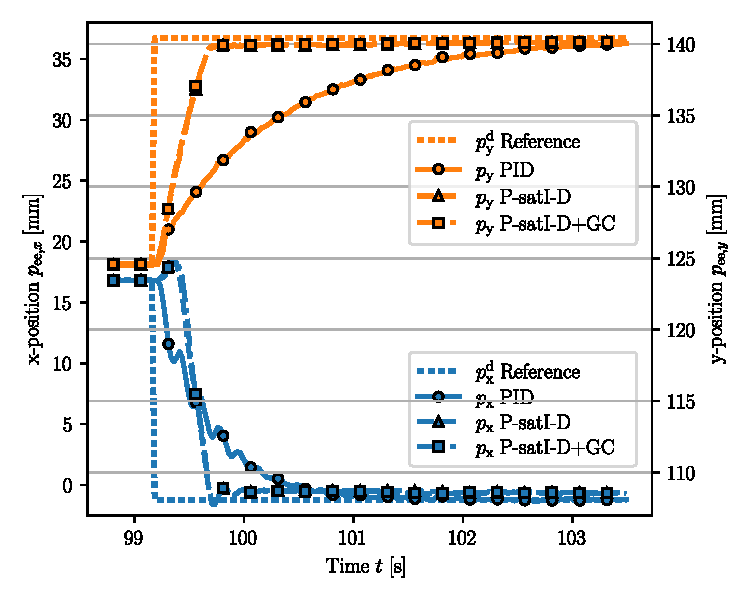
\includegraphics[width=0.47\columnwidth, trim={10, 10, 10, 10}]{hsacontrol/figures/experimental_results/epu/epu_step_response_chiee.pdf}\label{fig:hsacontrol:experimental_results:epu:step_response:pee}}
    \subfigure[Configuration]{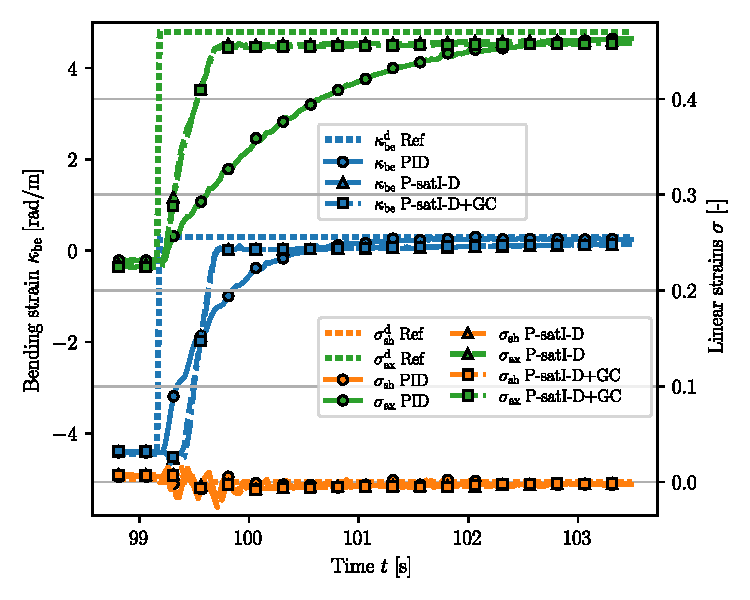
\includegraphics[width=0.47\columnwidth, trim={10, 10, 10, 10}]{hsacontrol/figures/experimental_results/epu/epu_step_response_q.pdf}\label{fig:hsacontrol:experimental_results:epu:step_response:q}}
    \caption{Step responses of the \emph{baseline PID}, \emph{P-satI-D} (with gravity compensation), and \emph{P-satI-D + GC} (with gravity cancellation) controllers on an EPU-based HSA robot.}\label{fig:hsacontrol:experimental_results:epu:step_response}
\end{figure}

\begin{figure}[ht]
    \centering
    \subfigure[End-effector position]{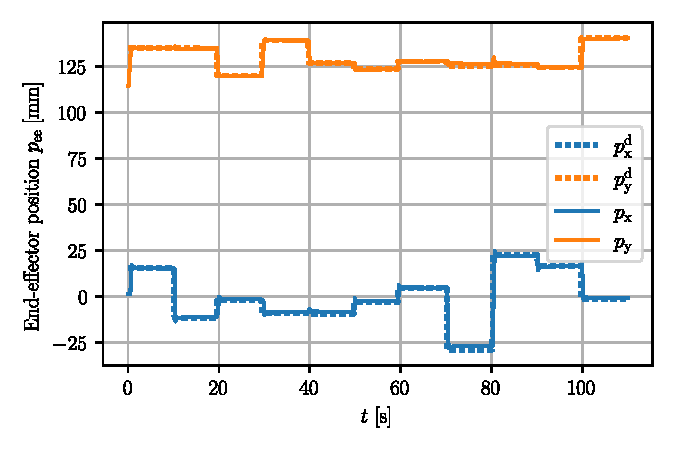
\includegraphics[width=0.49\columnwidth, trim={5, 10, 5, 5}]{hsacontrol/figures/experimental_results/epu/20231019_143126_pee.pdf}\label{fig:hsacontrol:experimental_results:epu:p_sati_d:pee}}
    \subfigure[Configuration]{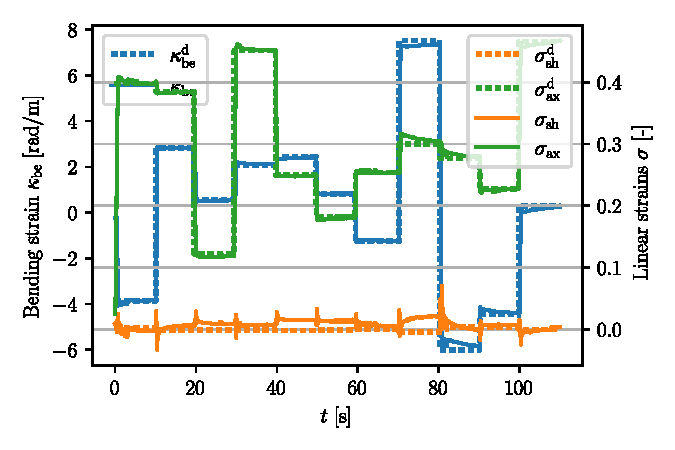
\includegraphics[width=0.49\columnwidth, trim={5, 10, 5, 5}]{hsacontrol/figures/experimental_results/epu/20231019_143126_q.pdf}\label{fig:hsacontrol:experimental_results:epu:p_sati_d:q}}\\
    \subfigure[Actuation coordinates]{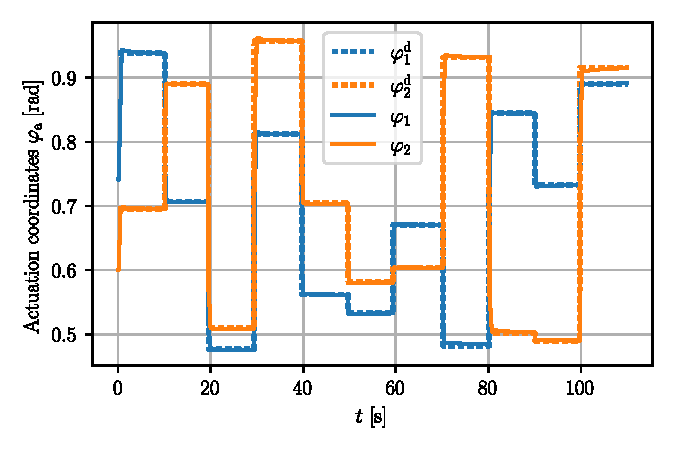
\includegraphics[width=0.49\columnwidth, trim={5, 10, 5, 5}]{hsacontrol/figures/experimental_results/epu/20231019_143126_varphi.pdf}\label{fig:hsacontrol:experimental_results:epu:p_sati_d:varphi}}
    \subfigure[Control input]{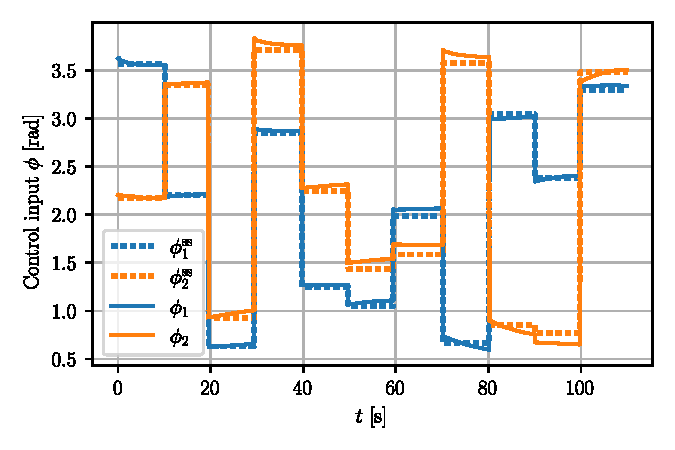
\includegraphics[width=0.49\columnwidth, trim={5, 10, 5, 5}]{hsacontrol/figures/experimental_results/epu/20231019_143126_phi.pdf}\label{fig:hsacontrol:experimental_results:epu:p_sati_d:phi}}
    \caption{Experimental results for tracking a reference trajectory of eleven step functions with the P-satI-D controller on an EPU-based HSA robot. \textbf{Panel (a):} End-effector position with the dotted and solid lines denoting the task-space reference and actual position, respectively.
    \textbf{Panel (b):} The planned (dotted) and the actual (solid) configuration. 
    \textbf{Panel (c):} The planned (dotted) and the actual (solid) actuation coordinates of the collocated system. 
    \textbf{Panel(d):} The saturated planar control inputs are visualized with solid lines, and the computed steady-state actuation with dotted lines.}\label{fig:hsacontrol:experimental_results:epu:p_sati_d}
\end{figure}

\subsubsection{Control of an EPU-based HSA robot}
Tracking the reference trajectory of eleven step functions with an EPU-based robot, the \emph{baseline PID} controller has an \gls{RMSE} of \SI{4.40}{mm}. The \emph{P-satI-D} (with gravity compensation) can able to achieve an \gls{RMSE} of \SI{3.63}{mm}. The \emph{P-satI-D + GC} controller exhibits similar performance(\gls{RMSE} of \SI{3.71}{mm}).
We visualize the step response of all three controllers in Fig.~\ref{fig:hsacontrol:experimental_results:epu:step_response} and the entire trajectory of the \emph{P-satI-D} controller in Fig.~\ref{fig:hsacontrol:experimental_results:epu:p_sati_d}.

Again, we notice that the response time of the model-based controllers (\SI{0.54}{s}) is much shorter than the response time of the baseline PID (\SI{3.84}{s}). Furthermore, the importance of a model-based control law is motivated by the oscillations in the transient of the baseline PID (see x-coordinate in Fig.~\ref{fig:hsacontrol:experimental_results:epu:step_response:pee}).
The steady-state error for the model-based controllers on the EPU material is slightly higher compared to the FPU material, as seen in Figures \ref{fig:hsacontrol:experimental_results:epu:step_response:pee} \& \ref{fig:hsacontrol:experimental_results:epu:p_sati_d:pee}. In Section~\ref{sub:hsacontrol:experiments:model_verification}, we noticed that the shear model doesn't fully capture the actual system behavior. This then results in an error in the planned desired configuration $q^\mathrm{d}$, which the controller is not able to resolve because of the underactuation of the robot (see Fig.~\ref{fig:hsacontrol:experimental_results:epu:p_sati_d:q}).
